\documentclass[aspectratio=169,10pt]{beamer}
\usepackage[utf8]{inputenc}
\usepackage[T1]{fontenc}
\usepackage{amsmath,amssymb,amsthm}
\usepackage{graphicx}
\usepackage{listings}
\usepackage{xcolor}
\usepackage{tikz}
\usepackage{algorithm}
\usepackage{algorithmic}
\usepackage{hyperref}
\usepackage{mimic}

\usetheme{Madrid}
\usecolortheme{seahorse}
\setbeamertemplate{navigation symbols}{}
\setbeamertemplate{footline}[frame number]

% Code listing configuration
\lstset{
    language=Python,
    basicstyle=\ttfamily\scriptsize,
    keywordstyle=\color{blue}\bfseries,
    stringstyle=\color{red},
    commentstyle=\color{green!60!black},
    showstringspaces=false,
    breaklines=true,
    breakatwhitespace=true,
    frame=single,
    numbers=left,
    numberstyle=\tiny\color{gray},
    xleftmargin=1em,
    framexleftmargin=1em
}

% Title page information
\title{Reinforcement Learning}
\subtitle{Lecture 4: Mathematical Foundations - MDPs and Bellman Equations}
\author{Taehoon Kim}
\institute{Sogang University MIMIC Lab \\ \url{https://mimic-lab.com}}
\date{Fall Semester 2025}

\begin{document}

% Slide 1: Title
\frame{\titlepage}


% Slide 3: Learning Objectives
\begin{frame}{Learning Objectives}
\textbf{By the end of this lecture, you will:}
\begin{enumerate}
    \item \textbf{Understand} the mathematical formulation of MDPs
    \item \textbf{Master} value functions and their recursive relationships
    \item \textbf{Derive} and apply Bellman equations
    \item \textbf{Implement} policy evaluation and improvement
    \item \textbf{Code} complete Policy Iteration and Value Iteration
    \item \textbf{Analyze} convergence properties and error bounds
\end{enumerate}

\vspace{0.5cm}
\textbf{Prerequisites:}
\begin{itemize}
    \item Linear algebra (matrix operations)
    \item Probability theory basics
    \item PyTorch tensor operations
    \item Python programming experience
\end{itemize}
\end{frame}

% Section 1: Introduction to MDPs
\section{Markov Decision Processes}

% Slide 4: What is an MDP?
\begin{frame}{What is a Markov Decision Process?}
\textbf{An MDP is a mathematical framework for sequential decision-making}

\vspace{0.5cm}
\textbf{Components:} $\mathcal{M} = (\mathcal{S}, \mathcal{A}, P, r, \gamma)$
\begin{itemize}
    \item $\mathcal{S}$: State space (finite or infinite)
    \item $\mathcal{A}$: Action space (finite or infinite)
    \item $P$: Transition dynamics $P(s' | s, a)$
    \item $r$: Reward function $r(s, a) = \mathbb{E}[R_{t+1} | S_t=s, A_t=a]$
    \item $\gamma$: Discount factor $\gamma \in [0, 1]$
\end{itemize}

\vspace{0.5cm}
\textbf{Key Property:} Markov Property
\begin{equation}
P(S_{t+1} | S_t, A_t, S_{t-1}, A_{t-1}, ...) = P(S_{t+1} | S_t, A_t)
\end{equation}
\end{frame}

% Slide 5: Agent-Environment Interaction (Simplified)
\begin{frame}{Agent-Environment Interaction}
\begin{center}
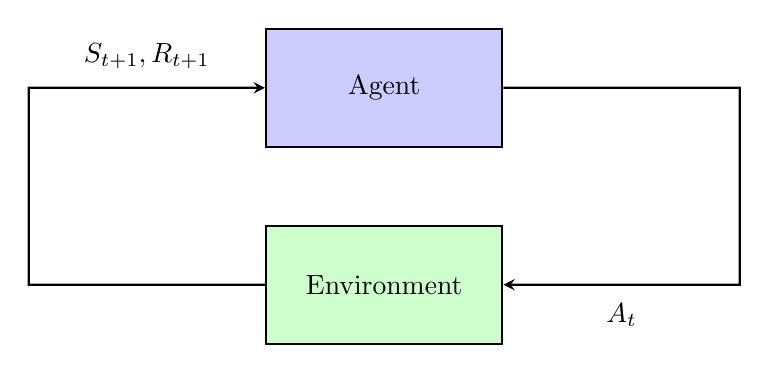
\begin{tikzpicture}[scale=1.0, node distance=2.5cm]
    % Styles
    \tikzstyle{box} = [rectangle, draw, thick, minimum width=3cm, minimum height=1.5cm, align=center]
    \tikzstyle{arrow} = [thick, ->, >=stealth]

    % Nodes
    \node[box, fill=blue!20] (agent) {Agent};
    \node[box, fill=green!20, below of=agent] (env) {Environment};

    % Arrows
    \draw[arrow] (agent.east) -- ++(3,0) -- ++(0,-2.5) -- (env.east) 
        node[midway, below=3pt] {$A_t$};

    \draw[arrow] (env.west) -- ++(-3,0) -- ++(0,2.5) -- (agent.west) 
        node[midway, above=3pt] {$S_{t+1}, R_{t+1}$};

\end{tikzpicture}
\end{center}

\vspace{0.5cm}
Trajectory: $S_0, A_0, R_1, S_1, A_1, R_2, S_2, \dots$
\end{frame}

% Slide 6: Example - GridWorld
\begin{frame}{Example: GridWorld MDP}
\begin{columns}
\column{0.5\textwidth}
\textbf{GridWorld Environment:}
\begin{itemize}
    \item States: Grid cells
    \item Actions: \{UP, RIGHT, DOWN, LEFT\}
    \item Transitions: Move to adjacent cell
    \item Rewards: -0.04 per step, +1 at goal, -1 at pit
    \item Discount: $\gamma = 0.99$
\end{itemize}

\column{0.5\textwidth}
\begin{center}
\begin{tabular}{|c|c|c|c|}
\hline
S & . & . & G(+1) \\
\hline
. & \# & . & P(-1) \\
\hline
. & . & . & . \\
\hline
\end{tabular}
\end{center}

\vspace{0.5cm}
S = Start, G = Goal, P = Pit, \# = Wall
\end{columns}
\end{frame}

% Slide 7: Transition Dynamics
\begin{frame}{Transition Dynamics}
\textbf{Deterministic vs Stochastic Transitions}

\begin{columns}
\column{0.5\textwidth}
\textbf{Deterministic:}
\begin{itemize}
    \item Action always leads to same next state
    \item $P(s' | s, a) \in \{0, 1\}$
    \item Simpler to analyze
\end{itemize}

\column{0.5\textwidth}
\textbf{Stochastic:}
\begin{itemize}
    \item Action may lead to different states
    \item $P(s' | s, a) \in [0, 1]$
    \item More realistic
\end{itemize}
\end{columns}

\vspace{0.5cm}
\textbf{Example with slip probability 0.2:}
\begin{itemize}
    \item Intended direction: probability 0.6
    \item Perpendicular directions: probability 0.2 each
\end{itemize}
\end{frame}

% Slide 8: Policies
\begin{frame}{Policies}
\textbf{A policy $\pi$ defines the agent's behavior}

\vspace{0.5cm}
\textbf{Types of Policies:}
\begin{itemize}
    \item \textbf{Deterministic:} $\pi: \mathcal{S} \rightarrow \mathcal{A}$
    \begin{itemize}
        \item Maps each state to a single action
        \item $a = \pi(s)$
    \end{itemize}
    \item \textbf{Stochastic:} $\pi: \mathcal{S} \times \mathcal{A} \rightarrow [0, 1]$
    \begin{itemize}
        \item Probability distribution over actions
        \item $\pi(a|s) = P(A_t = a | S_t = s)$
    \end{itemize}
\end{itemize}

\vspace{0.5cm}
\textbf{Goal:} Find the optimal policy $\pi^*$ that maximizes expected return
\end{frame}

% Slide 9: Returns and Episodes
\begin{frame}{Returns and Episodes}
\textbf{Return:} Sum of (discounted) future rewards

\vspace{0.5cm}
\textbf{Finite Horizon Return:}
\begin{equation}
G_t = R_{t+1} + R_{t+2} + ... + R_T
\end{equation}

\textbf{Infinite Horizon Discounted Return:}
\begin{equation}
G_t = \sum_{k=0}^{\infty} \gamma^k R_{t+k+1}
\end{equation}

\textbf{Why discount?}
\begin{itemize}
    \item Mathematical convergence
    \item Uncertainty about the future
    \item Economic interpretation (interest rates)
    \item Bounded returns: $|G_t| \leq \frac{R_{max}}{1-\gamma}$
\end{itemize}
\end{frame}

% Section 2: Value Functions
\section{Value Functions}

% Slide 10: State-Value Function
\begin{frame}{State-Value Function}
\textbf{Value of a state under policy $\pi$:}
\begin{equation}
v_\pi(s) = \mathbb{E}_\pi\left[\sum_{t=0}^{\infty} \gamma^t R_{t+1} \,\middle|\, S_0 = s\right]
\end{equation}

\textbf{Interpretation:}
\begin{itemize}
    \item Expected return starting from state $s$
    \item Following policy $\pi$ thereafter
    \item Accounts for all future rewards (discounted)
\end{itemize}

\textbf{Properties:}
\begin{itemize}
    \item Bounded: $|v_\pi(s)| \leq \frac{R_{max}}{1-\gamma}$
    \item Unique for a given policy and MDP
\end{itemize}
\end{frame}

% Slide 11: Action-Value Function
\begin{frame}{Action-Value Function (Q-Function)}
\textbf{Value of taking action $a$ in state $s$ under policy $\pi$:}
\begin{equation}
q_\pi(s, a) = \mathbb{E}_\pi\left[\sum_{t=0}^{\infty} \gamma^t R_{t+1} \,\middle|\, S_0 = s, A_0 = a\right]
\end{equation}

\textbf{Relationship to state-value:}
\begin{equation}
v_\pi(s) = \sum_a \pi(a|s) \, q_\pi(s, a)
\end{equation}

\textbf{Q-function tells us:}
\begin{itemize}
    \item How good is action $a$ in state $s$?
    \item Basis for action selection
    \item Central to Q-learning algorithms
\end{itemize}
\end{frame}

% Slide 12: Value Function Examples
\begin{frame}{Value Function Examples}
\begin{columns}
\column{0.5\textwidth}
\textbf{Random Policy Values:}
\begin{center}
\begin{tabular}{|c|c|c|c|}
\hline
0.52 & 0.55 & 0.61 & +1 \\
\hline
0.48 & \# & 0.43 & -1 \\
\hline
0.44 & 0.41 & 0.38 & 0.35 \\
\hline
\end{tabular}
\end{center}

\column{0.5\textwidth}
\textbf{Optimal Policy Values:}
\begin{center}
\begin{tabular}{|c|c|c|c|}
\hline
0.81 & 0.87 & 0.92 & +1 \\
\hline
0.76 & \# & 0.66 & -1 \\
\hline
0.71 & 0.66 & 0.61 & 0.39 \\
\hline
\end{tabular}
\end{center}
\end{columns}

\vspace{0.5cm}
\textbf{Observation:} Optimal values are higher (better policy)
\end{frame}

% Section 3: Bellman Expectation Equations
\section{Bellman Expectation Equations}

% Slide 13: Bellman Expectation for V
\begin{frame}{Bellman Expectation Equation for $v_\pi$}
\textbf{Recursive decomposition of value:}
\begin{equation}
v_\pi(s) = \mathbb{E}_\pi[R_{t+1} + \gamma v_\pi(S_{t+1}) | S_t = s]
\end{equation}

\textbf{Expanded form:}
\begin{equation}
v_\pi(s) = \sum_a \pi(a|s) \sum_{s'} P(s'|s,a) [r(s,a) + \gamma v_\pi(s')]
\end{equation}

\textbf{Key insight:}
\begin{itemize}
    \item Value = immediate reward + discounted future value
    \item Self-consistent system of equations
    \item One equation per state
\end{itemize}
\end{frame}

% Slide 14: Bellman Expectation for Q
\begin{frame}{Bellman Expectation Equation for $q_\pi$}
\textbf{Recursive decomposition:}
\begin{equation}
q_\pi(s,a) = r(s,a) + \gamma \sum_{s'} P(s'|s,a) \sum_{a'} \pi(a'|s') q_\pi(s',a')
\end{equation}

\textbf{Relationship between V and Q:}
\begin{align}
v_\pi(s) &= \sum_a \pi(a|s) q_\pi(s,a) \\
q_\pi(s,a) &= r(s,a) + \gamma \sum_{s'} P(s'|s,a) v_\pi(s')
\end{align}

\textbf{These equations form the basis for policy evaluation}
\end{frame}

% Slide 15: Matrix Form
\begin{frame}{Matrix Form of Bellman Expectation}
\textbf{For deterministic policy $\pi$:}

Define:
\begin{itemize}
    \item $\mathbf{v}_\pi \in \mathbb{R}^{|\mathcal{S}|}$: value vector
    \item $\mathbf{r}_\pi \in \mathbb{R}^{|\mathcal{S}|}$: reward vector
    \item $\mathbf{P}_\pi \in \mathbb{R}^{|\mathcal{S}| \times |\mathcal{S}|}$: transition matrix
\end{itemize}

\textbf{Bellman equation in matrix form:}
\begin{equation}
\mathbf{v}_\pi = \mathbf{r}_\pi + \gamma \mathbf{P}_\pi \mathbf{v}_\pi
\end{equation}

\textbf{Solution:}
\begin{equation}
\mathbf{v}_\pi = (\mathbf{I} - \gamma \mathbf{P}_\pi)^{-1} \mathbf{r}_\pi
\end{equation}

Note: Direct inversion is $O(n^3)$ - iterative methods preferred
\end{frame}

% Slide 16: Bellman Operator
\begin{frame}{Bellman Expectation Operator}
\textbf{Define operator $T_\pi: \mathbb{R}^{|\mathcal{S}|} \rightarrow \mathbb{R}^{|\mathcal{S}|}$:}
\begin{equation}
(T_\pi v)(s) = r_\pi(s) + \gamma \sum_{s'} P_\pi(s'|s) v(s')
\end{equation}

\textbf{Properties:}
\begin{itemize}
    \item $T_\pi$ is a $\gamma$-contraction in $\|\cdot\|_\infty$
    \item $\|T_\pi v - T_\pi w\|_\infty \leq \gamma \|v - w\|_\infty$
    \item Has unique fixed point $v_\pi$
    \item $v_\pi = T_\pi v_\pi$ (Bellman equation)
\end{itemize}

\textbf{Banach Fixed-Point Theorem:}
\begin{itemize}
    \item Starting from any $v_0$
    \item Sequence $v_{k+1} = T_\pi v_k$ converges to $v_\pi$
    \item Convergence rate: geometric with factor $\gamma$
\end{itemize}
\end{frame}

% Section 4: Bellman Optimality Equations
\section{Bellman Optimality Equations}

% Slide 17: Optimal Value Functions
\begin{frame}{Optimal Value Functions}
\textbf{Optimal state-value function:}
\begin{equation}
v_*(s) = \max_\pi v_\pi(s)
\end{equation}

\textbf{Optimal action-value function:}
\begin{equation}
q_*(s,a) = \max_\pi q_\pi(s,a)
\end{equation}

\textbf{Properties:}
\begin{itemize}
    \item Unique for a given MDP
    \item Defines the best possible performance
    \item Independent of initial state distribution
\end{itemize}

\textbf{Optimal policy:} Any policy achieving $v_*$ is optimal
\end{frame}

% Slide 18: Bellman Optimality Equation for V
\begin{frame}{Bellman Optimality Equation for $v_*$}
\textbf{The optimal value satisfies:}
\begin{equation}
v_*(s) = \max_a \left\{ r(s,a) + \gamma \sum_{s'} P(s'|s,a) v_*(s') \right\}
\end{equation}

\textbf{Key difference from expectation equation:}
\begin{itemize}
    \item Max over actions instead of expectation
    \item Non-linear due to max operator
    \item Harder to solve than expectation equation
\end{itemize}

\textbf{Interpretation:}
\begin{itemize}
    \item Optimal value = best immediate reward + discounted future
    \item Greedy action selection
\end{itemize}
\end{frame}

% Slide 19: Bellman Optimality Equation for Q
\begin{frame}{Bellman Optimality Equation for $q_*$}
\textbf{The optimal Q-function satisfies:}
\begin{equation}
q_*(s,a) = r(s,a) + \gamma \sum_{s'} P(s'|s,a) \max_{a'} q_*(s',a')
\end{equation}

\textbf{Relationship between $v_*$ and $q_*$:}
\begin{align}
v_*(s) &= \max_a q_*(s,a) \\
q_*(s,a) &= r(s,a) + \gamma \sum_{s'} P(s'|s,a) v_*(s')
\end{align}

\textbf{Optimal policy extraction:}
\begin{equation}
\pi_*(s) \in \arg\max_a q_*(s,a)
\end{equation}
\end{frame}

% Slide 20: Bellman Optimality Operator
\begin{frame}{Bellman Optimality Operator}
\textbf{Define operator $T_*: \mathbb{R}^{|\mathcal{S}|} \rightarrow \mathbb{R}^{|\mathcal{S}|}$:}
\begin{equation}
(T_* v)(s) = \max_a \left\{ r(s,a) + \gamma \sum_{s'} P(s'|s,a) v(s') \right\}
\end{equation}

\textbf{Properties:}
\begin{itemize}
    \item $T_*$ is a $\gamma$-contraction
    \item Unique fixed point $v_*$
    \item Monotonic: if $v \leq w$ then $T_* v \leq T_* w$
    \item Non-linear due to max
\end{itemize}

\textbf{Value Iteration:} $v_{k+1} = T_* v_k$ converges to $v_*$
\end{frame}

% Section 5: Dynamic Programming
\section{Dynamic Programming Algorithms}

% Slide 21: Dynamic Programming Overview
\begin{frame}{Dynamic Programming for MDPs}
\textbf{Requirements:}
\begin{itemize}
    \item Complete model of environment (P and r known)
    \item Finite state and action spaces
    \item Computational resources
\end{itemize}

\textbf{Two main algorithms:}
\begin{enumerate}
    \item \textbf{Policy Iteration:} Alternates evaluation and improvement
    \item \textbf{Value Iteration:} Directly applies optimality operator
\end{enumerate}

\textbf{Both algorithms:}
\begin{itemize}
    \item Converge to optimal policy
    \item Based on Bellman equations
    \item Exact solutions for finite MDPs
\end{itemize}
\end{frame}

% Slide 22: Policy Evaluation
\begin{frame}{Policy Evaluation}
\textbf{Given:} Policy $\pi$, MDP model \\
\textbf{Find:} $v_\pi$

\begin{algorithm}[H]
\caption{Iterative Policy Evaluation}
\begin{algorithmic}[1]
\STATE Initialize $V(s) = 0$ for all $s \in \mathcal{S}$
\REPEAT
    \STATE $\Delta \leftarrow 0$
    \FOR{each $s \in \mathcal{S}$}
        \STATE $v \leftarrow V(s)$
        \STATE $V(s) \leftarrow \sum_a \pi(a|s) \sum_{s'} P(s'|s,a)[r(s,a) + \gamma V(s')]$
        \STATE $\Delta \leftarrow \max(\Delta, |v - V(s)|)$
    \ENDFOR
\UNTIL{$\Delta < \epsilon$}
\RETURN $V$
\end{algorithmic}
\end{algorithm}
\end{frame}

% Slide 23: Policy Improvement
\begin{frame}{Policy Improvement}
\textbf{Given:} Value function $v_\pi$ \\
\textbf{Find:} Better policy $\pi'$

\textbf{Greedy policy with respect to $v_\pi$:}
\begin{equation}
\pi'(s) = \arg\max_a \left\{ r(s,a) + \gamma \sum_{s'} P(s'|s,a) v_\pi(s') \right\}
\end{equation}

\textbf{Policy Improvement Theorem:}
\begin{itemize}
    \item If $\pi'$ is greedy w.r.t. $v_\pi$
    \item Then $v_{\pi'}(s) \geq v_\pi(s)$ for all $s$
    \item Equality holds iff $\pi$ is optimal
\end{itemize}

\textbf{This guarantees monotonic improvement!}
\end{frame}

% Slide 24: Policy Iteration Algorithm
\begin{frame}{Policy Iteration}
\begin{algorithm}[H]
\caption{Policy Iteration}
\begin{algorithmic}[1]
\STATE Initialize $\pi$ arbitrarily
\REPEAT
    \STATE \textbf{Policy Evaluation:}
    \STATE \quad Compute $v_\pi$ using iterative evaluation
    \STATE \textbf{Policy Improvement:}
    \STATE \quad $\pi_{old} \leftarrow \pi$
    \FOR{each $s \in \mathcal{S}$}
        \STATE $\pi(s) \leftarrow \arg\max_a q_\pi(s,a)$
    \ENDFOR
\UNTIL{$\pi = \pi_{old}$}
\RETURN $\pi$
\end{algorithmic}
\end{algorithm}

\textbf{Convergence:} Finite number of iterations for finite MDPs
\end{frame}

% Slide 25: Value Iteration Algorithm
\begin{frame}{Value Iteration}
\begin{algorithm}[H]
\caption{Value Iteration}
\begin{algorithmic}[1]
\STATE Initialize $V(s) = 0$ for all $s \in \mathcal{S}$
\REPEAT
    \STATE $\Delta \leftarrow 0$
    \FOR{each $s \in \mathcal{S}$}
        \STATE $v \leftarrow V(s)$
        \STATE $V(s) \leftarrow \max_a \sum_{s'} P(s'|s,a)[r(s,a) + \gamma V(s')]$
        \STATE $\Delta \leftarrow \max(\Delta, |v - V(s)|)$
    \ENDFOR
\UNTIL{$\Delta < \epsilon$}
\STATE Extract policy: $\pi(s) = \arg\max_a q(s,a)$
\RETURN $\pi$
\end{algorithmic}
\end{algorithm}

\textbf{Combines evaluation and improvement in single update}
\end{frame}

% Slide 26: PI vs VI Comparison
\begin{frame}{Policy Iteration vs Value Iteration}
\begin{center}
\begin{tabular}{|l|l|l|}
\hline
\textbf{Aspect} & \textbf{Policy Iteration} & \textbf{Value Iteration} \\
\hline
Updates & Alternating & Combined \\
Convergence & Fewer iterations & More iterations \\
Per iteration cost & Higher (full evaluation) & Lower (single backup) \\
Memory & Store policy + values & Store values only \\
Early stopping & Natural (policy stable) & Needs error bound \\
Implementation & More complex & Simpler \\
\hline
\end{tabular}
\end{center}

\vspace{0.5cm}
\textbf{In practice:}
\begin{itemize}
    \item VI often preferred for simplicity
    \item PI can be faster for some problems
    \item Modified PI: partial evaluation
\end{itemize}
\end{frame}

% Section 6: Convergence and Complexity
\section{Convergence and Complexity}

% Slide 27: Contraction Mapping
\begin{frame}{Contraction Mapping Theorem}
\textbf{Theorem:} If $T$ is a $\gamma$-contraction on complete metric space, then:
\begin{enumerate}
    \item $T$ has unique fixed point $v^*$
    \item For any $v_0$, sequence $v_{k+1} = Tv_k$ converges to $v^*$
    \item $\|v_k - v^*\|_\infty \leq \gamma^k \|v_0 - v^*\|_\infty$
\end{enumerate}

\textbf{Application to RL:}
\begin{itemize}
    \item Both $T_\pi$ and $T_*$ are contractions
    \item Guarantees convergence of DP algorithms
    \item Provides convergence rate
\end{itemize}

\textbf{Convergence rate:}
\begin{itemize}
    \item Geometric with factor $\gamma$
    \item Higher $\gamma$ → slower convergence
    \item Number of iterations $\propto \frac{1}{1-\gamma}$
\end{itemize}
\end{frame}

% Slide 28: Error Bounds
\begin{frame}{Error Bounds for Value Iteration}
\textbf{After $k$ iterations of value iteration:}
\begin{equation}
\|V_k - v_*\|_\infty \leq \gamma^k \|V_0 - v_*\|_\infty
\end{equation}

\textbf{Using Bellman residual $\delta_k = \|V_{k+1} - V_k\|_\infty$:}
\begin{equation}
\|V_k - v_*\|_\infty \leq \frac{\gamma}{1-\gamma} \delta_k
\end{equation}

\textbf{Stopping criterion for $\epsilon$-optimal solution:}
\begin{itemize}
    \item Want: $\|V_k - v_*\|_\infty \leq \epsilon$
    \item Stop when: $\delta_k < \frac{(1-\gamma)\epsilon}{2\gamma}$
\end{itemize}

\textbf{These bounds are tight and computable!}
\end{frame}

% Slide 29: Computational Complexity
\begin{frame}{Computational Complexity}
\textbf{Per iteration complexity:}
\begin{itemize}
    \item Policy Evaluation: $O(|\mathcal{S}|^2 |\mathcal{A}|)$ per iteration
    \item Policy Improvement: $O(|\mathcal{S}|^2 |\mathcal{A}|)$
    \item Value Iteration: $O(|\mathcal{S}|^2 |\mathcal{A}|)$ per iteration
\end{itemize}

\textbf{Number of iterations:}
\begin{itemize}
    \item Policy Iteration: $O(|\mathcal{A}|^{|\mathcal{S}|})$ worst case (rarely reached)
    \item Value Iteration: $O(\frac{1}{1-\gamma} \log \frac{1}{\epsilon})$
\end{itemize}

\textbf{Space complexity:}
\begin{itemize}
    \item Transition matrix: $O(|\mathcal{S}|^2 |\mathcal{A}|)$
    \item Value function: $O(|\mathcal{S}|)$
    \item Policy: $O(|\mathcal{S}|)$
\end{itemize}
\end{frame}

% Section 7: Implementation
\section{PyTorch Implementation}

% Slide 30: Setup and Imports
\begin{frame}[fragile]{Implementation: Setup}
\begin{lstlisting}
import torch
import numpy as np

def setup_seed(seed=42):
    torch.manual_seed(seed)
    np.random.seed(seed)
    if torch.cuda.is_available():
        torch.cuda.manual_seed_all(seed)

device = torch.device(
    'cuda' if torch.cuda.is_available()
    else 'mps' if torch.backends.mps.is_available()
    else 'cpu'
)

# MDP components shapes
# P: [S, A, S] - transition probabilities
# R: [S, A]    - rewards
# V: [S]       - values
# Q: [S, A]    - Q-values
# pi: [S]      - deterministic policy
\end{lstlisting}
\end{frame}

% Slide 31: GridWorld MDP Class
\begin{frame}[fragile]{GridWorld MDP Implementation}
\begin{lstlisting}
class GridWorldMDP:
    def __init__(self, grid, terminal_rewards, 
                 step_cost=-0.04, slip_prob=0.1):
        self.height = len(grid)
        self.width = len(grid[0])
        
        # Build state mapping
        self.state_to_pos = {}
        self.pos_to_state = {}
        state_idx = 0
        for r in range(self.height):
            for c in range(self.width):
                if grid[r][c] != '#':  # Not a wall
                    self.state_to_pos[state_idx] = (r, c)
                    self.pos_to_state[(r, c)] = state_idx
                    state_idx += 1
        
        self.n_states = len(self.state_to_pos)
        self.n_actions = 4  # UP, RIGHT, DOWN, LEFT
\end{lstlisting}
\end{frame}

% Slide 32: Building Transition Matrix
\begin{frame}[fragile]{Building Transition and Reward Matrices}
\begin{lstlisting}
def build_dynamics(self):
    P = torch.zeros((self.n_states, self.n_actions, 
                     self.n_states), device=device)
    R = torch.full((self.n_states, self.n_actions), 
                   self.step_cost, device=device)
    
    for s in range(self.n_states):
        if self.is_terminal[s]:
            P[s, :, s] = 1.0  # Absorbing state
            R[s, :] = 0.0
            continue
        
        for a in range(self.n_actions):
            # Stochastic transitions with slip
            for actual_a, prob in self.get_transitions(a):
                next_s = self.get_next_state(s, actual_a)
                P[s, a, next_s] += prob
                R[s, a] += prob * self.get_reward(next_s)
    
    return P, R
\end{lstlisting}
\end{frame}

% Slide 33: Policy Evaluation Implementation
\begin{frame}[fragile]{Policy Evaluation in PyTorch}
\begin{lstlisting}
def policy_evaluation(P, R, pi, gamma=0.99, tol=1e-8):
    """Evaluate a policy using matrix operations"""
    S = P.shape[0]
    
    # Convert policy to transition matrix
    if pi.dim() == 1:  # Deterministic
        P_pi = P[torch.arange(S), pi]  # [S, S]
        R_pi = R[torch.arange(S), pi]  # [S]
    else:  # Stochastic
        P_pi = torch.einsum('sa,sas->ss', pi, P)
        R_pi = torch.einsum('sa,sa->s', pi, R)
    
    V = torch.zeros(S, device=P.device)
    
    for _ in range(1000):
        V_new = R_pi + gamma * (P_pi @ V)
        if torch.max(torch.abs(V_new - V)) < tol:
            break
        V = V_new
    
    return V
\end{lstlisting}
\end{frame}

% Slide 34: Policy Improvement Implementation
\begin{frame}[fragile]{Policy Improvement in PyTorch}
\begin{lstlisting}
def policy_improvement(P, R, V, gamma=0.99):
    """Extract greedy policy from value function"""
    # Compute Q-values
    # Q(s,a) = R(s,a) + gamma * sum_s' P(s,a,s') * V(s')
    Q = R + gamma * torch.einsum('sas,s->sa', P, V)
    
    # Extract greedy policy
    pi = torch.argmax(Q, dim=1)
    
    return pi, Q

def compute_q_values(P, R, V, gamma=0.99):
    """Compute Q-values from value function"""
    return R + gamma * torch.einsum('sas,s->sa', P, V)
\end{lstlisting}
\end{frame}

% Slide 35: Policy Iteration Implementation
\begin{frame}[fragile]{Complete Policy Iteration}
\begin{lstlisting}
def policy_iteration(P, R, gamma=0.99, tol=1e-8):
    S, A = P.shape[0], P.shape[1]
    pi = torch.zeros(S, dtype=torch.long)  # Start arbitrary
    
    for iteration in range(100):
        # Policy Evaluation
        V = policy_evaluation(P, R, pi, gamma, tol)
        
        # Policy Improvement
        pi_new, Q = policy_improvement(P, R, V, gamma)
        
        # Check convergence
        if torch.equal(pi_new, pi):
            print(f"Converged in {iteration + 1} iterations")
            break
        
        pi = pi_new
    
    return pi, V
\end{lstlisting}
\end{frame}

% Slide 36: Value Iteration Implementation
\begin{frame}[fragile]{Value Iteration in PyTorch}
\begin{lstlisting}
def value_iteration(P, R, gamma=0.99, tol=1e-8):
    S = P.shape[0]
    V = torch.zeros(S, device=P.device)
    
    for iteration in range(1000):
        V_old = V.clone()
        
        # Bellman optimality update
        Q = compute_q_values(P, R, V_old, gamma)
        V = torch.max(Q, dim=1)[0]
        
        # Check convergence
        delta = torch.max(torch.abs(V - V_old))
        if delta < tol:
            print(f"Converged in {iteration + 1} iterations")
            break
    
    # Extract optimal policy
    Q_final = compute_q_values(P, R, V, gamma)
    pi = torch.argmax(Q_final, dim=1)
    
    return pi, V
\end{lstlisting}
\end{frame}

% Section 8: Experiments
\section{Hands-on Experiments}

% Slide 37: Experiment 1 - Environment Setup
\begin{frame}{Experiment 1: Environment Setup}
\textbf{File:} \texttt{exp01\_setup.py}

\textbf{Objectives:}
\begin{itemize}
    \item Verify PyTorch installation
    \item Test device selection (CUDA/MPS/CPU)
    \item Initialize MDP tensors
    \item Verify tensor shapes and operations
\end{itemize}

\textbf{Key checks:}
\begin{itemize}
    \item Transition probabilities sum to 1
    \item Reward bounds are finite
    \item Bellman operator properties
\end{itemize}

\textbf{Expected output:} System info, device selection, tensor verification
\end{frame}

% Slide 38: Experiment 2 - GridWorld
\begin{frame}{Experiment 2: GridWorld MDP}
\textbf{File:} \texttt{exp02\_gridworld.py}

\textbf{Tasks:}
\begin{itemize}
    \item Build complete GridWorld environment
    \item Create transition matrix P[s,a,s']
    \item Create reward matrix R[s,a]
    \item Handle walls and terminal states
    \item Add stochastic transitions (slip)
\end{itemize}

\textbf{Verification:}
\begin{itemize}
    \item P matrix: proper probability distribution
    \item Terminal states are absorbing
    \item Transitions respect walls
\end{itemize}
\end{frame}

% Slide 39: Experiment 3 - Policy Evaluation
\begin{frame}{Experiment 3: Policy Evaluation}
\textbf{File:} \texttt{exp03\_policy\_evaluation.py}

\textbf{Implement and test:}
\begin{itemize}
    \item Iterative policy evaluation
    \item Contraction property verification
    \item Compare different policies (random, fixed)
    \item Analyze convergence rates with different $\gamma$
\end{itemize}

\textbf{Key observations:}
\begin{itemize}
    \item Geometric convergence
    \item Higher $\gamma$ → slower convergence
    \item Unique fixed point
\end{itemize}
\end{frame}

% Slide 40: Experiment 4 - Policy Improvement
\begin{frame}{Experiment 4: Policy Improvement}
\textbf{File:} \texttt{exp04\_policy\_improvement.py}

\textbf{Tasks:}
\begin{itemize}
    \item Compute Q-values from V
    \item Extract greedy policy
    \item Verify improvement theorem
    \item Compare deterministic vs soft improvement
\end{itemize}

\textbf{Verification:}
\begin{itemize}
    \item $v_{\pi'} \geq v_\pi$ for all states
    \item Monotonic improvement
    \item Convergence to optimal
\end{itemize}
\end{frame}

% Slide 41: Experiment 5 - Policy Iteration
\begin{frame}{Experiment 5: Policy Iteration}
\textbf{File:} \texttt{exp05\_policy\_iteration.py}

\textbf{Complete implementation:}
\begin{itemize}
    \item Full policy iteration algorithm
    \item Track policy evolution
    \item Compare different initial policies
    \item Visualize convergence
\end{itemize}

\textbf{Analysis:}
\begin{itemize}
    \item Number of iterations to convergence
    \item Policy changes per iteration
    \item Final optimal policy
\end{itemize}
\end{frame}

% Slide 42: Experiment 6 - Value Iteration
\begin{frame}{Experiment 6: Value Iteration}
\textbf{File:} \texttt{exp06\_value\_iteration.py}

\textbf{Implement:}
\begin{itemize}
    \item Value iteration algorithm
    \item Compare with policy iteration
    \item Test different initializations
    \item Analyze Bellman optimality operator
\end{itemize}

\textbf{Comparisons:}
\begin{itemize}
    \item VI vs PI convergence speed
    \item Computational efficiency
    \item Memory requirements
\end{itemize}
\end{frame}

% Slide 43: Experiment 7 - Stopping Criteria
\begin{frame}{Experiment 7: Stopping Criteria}
\textbf{File:} \texttt{exp07\_stopping\_criteria.py}

\textbf{Explore:}
\begin{itemize}
    \item Different stopping criteria
    \item Error bounds computation
    \item Trade-offs: accuracy vs computation
    \item Early stopping strategies
\end{itemize}

\textbf{Key results:}
\begin{itemize}
    \item Theoretical bounds are tight
    \item Policy often converges before values
    \item Span seminorm alternative
\end{itemize}
\end{frame}

% Slide 44: Experiment 8 - Optimizations
\begin{frame}{Experiment 8: Algorithmic Optimizations}
\textbf{File:} \texttt{exp08\_optimizations.py}

\textbf{Compare:}
\begin{itemize}
    \item Synchronous vs asynchronous updates
    \item Prioritized sweeping
    \item GPU acceleration
    \item Memory efficiency
\end{itemize}

\textbf{Performance metrics:}
\begin{itemize}
    \item Iterations to convergence
    \item Wall-clock time
    \item Memory usage
    \item Scalability
\end{itemize}
\end{frame}

% Slide 45: Experiment 9 - Integration Test
\begin{frame}{Experiment 9: Integrated Test}
\textbf{File:} \texttt{exp09\_integrated\_test.py}

\textbf{Complete pipeline:}
\begin{itemize}
    \item Multiple test scenarios
    \item All algorithms comparison
    \item Comprehensive visualization
    \item Performance benchmarking
\end{itemize}

\textbf{Deliverables:}
\begin{itemize}
    \item Optimal policies for each scenario
    \item Algorithm comparison report
    \item Convergence verification
    \item Reproducibility guarantee
\end{itemize}
\end{frame}



% Section 13: Summary
\section{Summary and Next Steps}

% Slide 59: Key Takeaways
\begin{frame}{Key Takeaways}
\textbf{Theory:}
\begin{itemize}
    \item MDPs provide mathematical framework for sequential decisions
    \item Value functions satisfy Bellman equations
    \item Bellman operators are contractions → unique solutions
    \item DP algorithms solve MDPs exactly
\end{itemize}

\textbf{Practice:}
\begin{itemize}
    \item Implemented complete GridWorld MDP
    \item Policy evaluation converges geometrically
    \item Policy improvement guarantees monotonic improvement
    \item PI and VI converge to same optimal policy
\end{itemize}

\textbf{Insights:}
\begin{itemize}
    \item Model-based methods are sample efficient
    \item Computation scales with state/action space
    \item Foundation for model-free methods
\end{itemize}
\end{frame}

% Slide 61: Mathematical Foundations Summary
\begin{frame}{Mathematical Foundations Summary}
\begin{center}
\begin{tabular}{|l|l|}
\hline
\textbf{Concept} & \textbf{Key Equation} \\
\hline
State Value & $v_\pi(s) = \mathbb{E}_\pi[G_t | S_t = s]$ \\
Action Value & $q_\pi(s,a) = \mathbb{E}_\pi[G_t | S_t = s, A_t = a]$ \\
Bellman Expectation & $v_\pi = r_\pi + \gamma P_\pi v_\pi$ \\
Bellman Optimality & $v_* = \max_a \{r_a + \gamma P_a v_*\}$ \\
Policy Evaluation & $v_{k+1} = T_\pi v_k$ \\
Value Iteration & $v_{k+1} = T_* v_k$ \\
Greedy Policy & $\pi(s) = \arg\max_a q(s,a)$ \\
\hline
\end{tabular}
\end{center}

\textbf{Remember:} These equations are the heart of RL!
\end{frame}


\end{document}